% 请确保文件编码为utf-8,使用XeLaTex进行编译,或者通过overleaf进行编译

\documentclass[answers]{exam}  % 使用此行带有作答模块
% \documentclass{exam} % 使用此行只显示题目

\usepackage{xeCJK}
\usepackage{zhnumber}
\usepackage{graphicx}
\usepackage{hyperref}
\usepackage{amsmath}
\usepackage{booktabs}
\usepackage{enumerate}
\usepackage{amssymb}
\usepackage{listings}
\usepackage{floatrow}
\usepackage{blindtext}
\usepackage{subcaption}
\pagestyle{headandfoot}
\firstpageheadrule
\firstpageheader{南京大学}{机器学习导论}{习题四}
\runningheader{南京大学}
{机器学习导论}
{习题四}
\runningheadrule
\firstpagefooter{}{第\thepage\ 页(共\numpages 页)}{}
\runningfooter{}{第\thepage\ 页(共\numpages 页)}{}


\setlength\linefillheight{.5in}

\renewcommand{\solutiontitle}{\noindent\textbf{解:}\par\noindent}

\renewcommand{\thequestion}{\zhnum{question}}
\renewcommand{\questionlabel}{\thequestion .}
\renewcommand{\thepartno}{\arabic{partno}}
\renewcommand{\partlabel}{\thepartno .}

\lstset{language=Matlab}%这条命令可以让LaTeX排版时将Matlab关键字突出显示
\lstset{
	breaklines,%这条命令可以让LaTeX自动将长的代码行换行排版
	basicstyle=\footnotesize\ttfamily, % Standardschrift
	backgroundcolor=\color[rgb]{0.95,0.95,0.95},
	keywordstyle=\color{blue},
	commentstyle=\color{cyan},
	tabsize=4,numbers=left,
	numberstyle=\tiny,
	frame=single,
	%numbers=left, % Ort der Zeilennummern
	numberstyle=\tiny, % Stil der Zeilennummern
	%stepnumber=2, % Abstand zwischen den Zeilennummern
	numbersep=5pt, % Abstand der Nummern zum Text
	tabsize=2, % Groesse von Tabs
	extendedchars=false, %
	breaklines=true, % Zeilen werden Umgebrochen
	keywordstyle=\color{red},%这一条命令可以解决代码跨页时, 章节标题, 页眉等汉字不显示的问题
	stringstyle=\color{white}\ttfamily, % Farbe der String
	showspaces=false, % Leerzeichen anzeigen ?
	showtabs=false, % Tabs anzeigen ?
	xleftmargin=17pt,
	framexleftmargin=17pt,
	framexrightmargin=5pt,
	framexbottommargin=4pt,
	%backgroundcolor=\color{lightgray},
	showstringspaces=false % Leerzeichen in Strings anzeigen ?
}
\renewcommand{\lstlistingname}{CODE}
\lstloadlanguages{% Check Dokumentation for further languages ...
	%[Visual]Basic
	%Pascal
	%C
	Python
	%XML
	%HTML
	%Java
}
%%% load AMS-Latex Package
\usepackage{amssymb}
\usepackage{amsmath,amsfonts}
% \usepackage{amsthm}
\usepackage{amsopn}
\usepackage{bm} % bold symbol
\usepackage{multirow}



% operator in optimization
\DeclareMathOperator{\argmax}{arg\,max}
\DeclareMathOperator{\argmin}{arg\,min}
\DeclareMathOperator{\softmax}{softmax}

% special functions
\newcommand{\trace}[1]{\operatornamewithlimits{tr}\left\{#1\right\}}
\newcommand{\diag}{\operatornamewithlimits{diag}}
\newcommand{\sign}{\operatornamewithlimits{sign}}
\newcommand{\const}{\operatornamewithlimits{const}}

% special display
\newcommand{\parde}[2]{\frac{\partial #1}{\partial  #2}}

% define vector and matrix symbols
\newcommand{\vct}[1]{\boldsymbol{#1}} % vector
\newcommand{\mat}[1]{\boldsymbol{#1}} % matrix
\newcommand{\cst}[1]{\mathsf{#1}}  % constant

% shorthand
\newcommand{\vtheta}{\vct{\theta}}
\newcommand{\vmu}{\vct{\mu}}
\newcommand{\vc}{\vct{c}}
\newcommand{\vp}{\vct{p}}
\newcommand{\vq}{\vct{q}}
\newcommand{\vx}{{\vct{x}}}
\newcommand{\vy}{\vct{y}}
\newcommand{\vz}{{\vct{z}}}
\newcommand{\vu}{\vct{u}}
\newcommand{\vo}{{\vct{o}}}
\newcommand{\va}{\vct{a}}
\newcommand{\vb}{\vct{b}}
\newcommand{\ve}{\vct{e}}
\newcommand{\vr}{\vct{r}}
\newcommand{\vt}{\vct{t}}
%\newcommand{\vpsi}{\vct{\psi}}
\newcommand{\vs}{\vct{s}}
\newcommand{\vv}{\vct{v}}
\newcommand{\vw}{\vct{w}}
\newcommand{\vzero}{\vct{0}}
\newcommand{\vf}{\vct{f}}
\newcommand{\vh}{\vct{h}}
\newcommand{\vg}{\vct{g}}
\newcommand{\vphi}{\vct{\phi}}
\newcommand{\vpsi}{\vct{\psi}}
\newcommand{\ones}{\vct{1}}
\newcommand{\mU}{\mat{U}}
\newcommand{\mA}{\mat{A}}
\newcommand{\mB}{\mat{B}}
\newcommand{\mC}{\mat{C}}
\newcommand{\mD}{\mat{D}}
\newcommand{\mV}{\mat{V}}
\newcommand{\mW}{\mat{W}}
\newcommand{\mH}{\mat{H}}
\newcommand{\mI}{\mat{I}}
\newcommand{\mP}{\mat{P}}
\newcommand{\mS}{\mat{S}}
\newcommand{\mJ}{\mat{J}}
\newcommand{\mM}{\mat{M}}
\newcommand{\mT}{\mat{T}}
\newcommand{\mZ}{\mat{Z}}
\newcommand{\mO}{\mat{O}}
\newcommand{\mX}{\mat{X}}
\newcommand{\mY}{\mat{Y}}
\newcommand{\mQ}{\mat{Q}}
\newcommand{\mLambda}{\mat{\Lambda}}
% \newcommand{\mL}{\mat{L}}
\newcommand{\mmI}{\mat{I}}
\newcommand{\mK}{\mat{K}}
\newcommand{\mSigma}{\mat{\Sigma}}
\newcommand{\mOmega}{\mat{\Omega}}
\newcommand{\cC}{\cst{C}}
\newcommand{\cM}{\cst{M}}
\newcommand{\cN}{\cst{N}}
\newcommand{\cQ}{\cst{Q}}
\newcommand{\cD}{\cst{D}}
\newcommand{\cL}{\cst{L}}
\newcommand{\cK}{\cst{K}}
\newcommand{\cH}{\cst{H}}
\newcommand{\cR}{\cst{R}}
\newcommand{\cU}{\cst{U}}
\newcommand{\cS}{\cst{S}}
\newcommand{\cX}{\cst{X}}
\newcommand{\sQ}{\mathcal{Q}}
\newcommand{\sS}{\mathcal{S}}
\newcommand{\sF}{\mathcal{F}}
\newcommand{\sC}{\mathcal{C}}
\newcommand{\sX}{\mathcal{X}}
\newcommand{\sH}{\mathcal{H}}

\newcommand{\bE}{\mathbb{E}}
\newcommand{\bR}{\mathbb{R}}
\newcommand{\bH}{\mathbb{H}}

\usepackage{algorithm}  
% \usepackage{algorithmic}
%\usepackage{algorithmicx}  
\usepackage{algpseudocode}  

\floatname{algorithm}{算法}  
\renewcommand{\algorithmicrequire}{\textbf{输入:}}  
\renewcommand{\algorithmicensure}{\textbf{输出:}}  

\begin{document}
\Large
\noindent 
% 姓名学号
姓名:杜兴豪 \\
学号:201300096\\
\begin{questions}
\question [20] \textbf{神经网络基础} \\

给定训练集$D=\{(\vx_1, \vy_1), (\vx_2, \vy_2), ..., (\vx_m, \vy_m)\}$. 其中$\vx_i \in \bR^d$,
$\vy_i \in \bR^l$表示输入示例由$d$个属性描述,
输出$l$维实值向量.
图~\ref{ch5_img:mlp}给出了一个有$d$个输入神经元、$l$个输出神经元、$q$个隐层神经元的多层神经网络, 其中输出层第$j$个神经元的阈值用$\theta_j$表示, 隐层第$h$个神经元的阈值用$\gamma_h$表示. 输入层第$i$个神经元与隐层第$h$个神经元之间的连接权为$v_{ih}$,
隐层第$h$个神经元与输出层第$j$个神经元之间的连接权为$w_{hj}$.
记隐层第$h$个神经元接收到的输入为$\alpha_h=\sum_{i=1}^d v_{ih}x_i$,
输出层第$j$个神经元接收到的输入为$\beta_j=\sum_{h=1}^q w_{hj}b_h$,
其中$b_h$为隐层第$h$个神经元的输出.
\begin{figure}[ht]
    \centering
    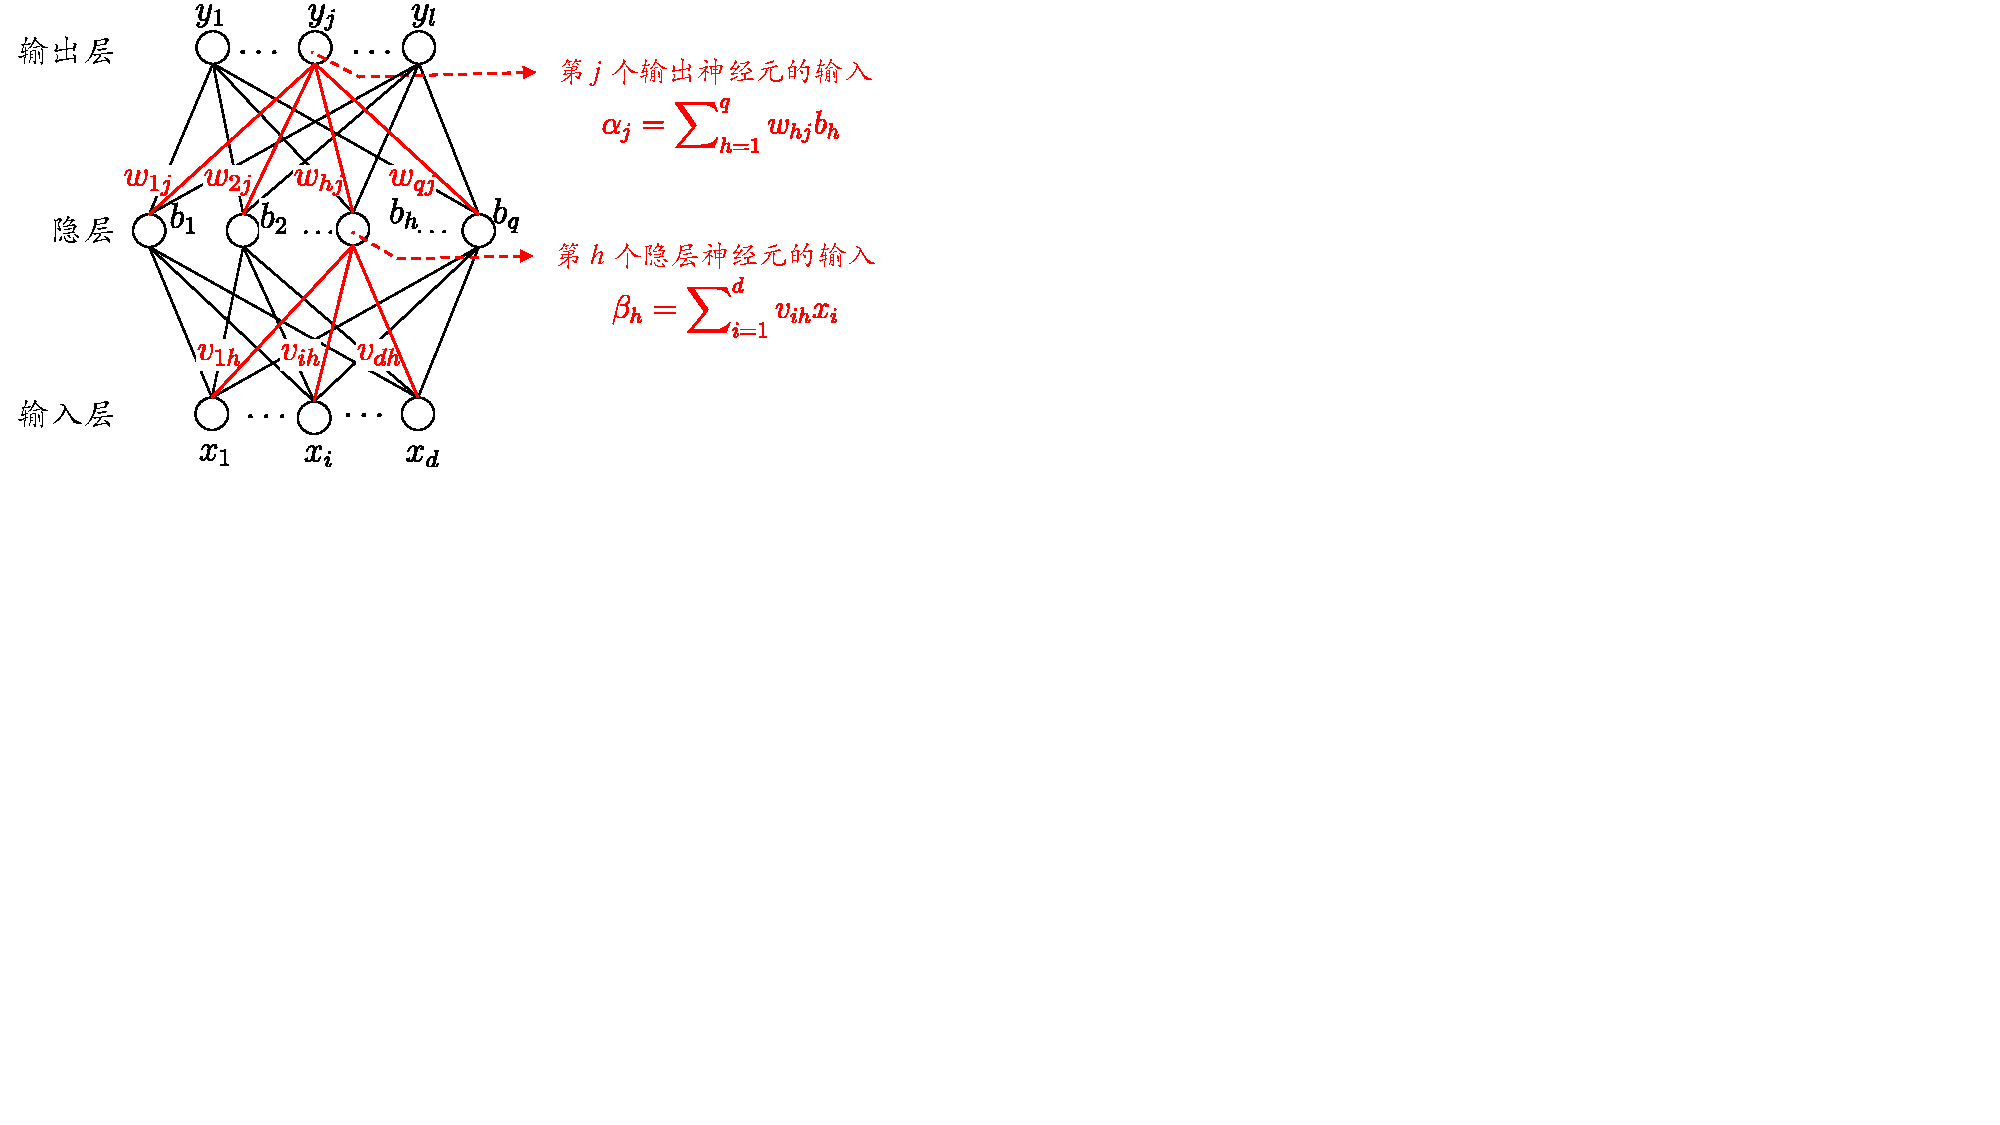
\includegraphics[width=0.70\textwidth]{figure/ch5_nn.pdf}
    \caption{多层神经网络(教材图5.7)}\label{ch5_img:mlp}
\end{figure}

不同任务中神经网络的输出层往往使用不同的激活函数和损失函数,
本题介绍几种常见的激活和损失函数, 并对其梯度进行推导.
\begin{enumerate}
    \item 在二分类问题中($l=1$), 标记$y\in\{0,1\}$, 一般使用Sigmoid函数作为激活函数,
    使输出值在$[0, 1]$范围内, 使模型预测结果可直接作为概率输出.
    Sigmoid函数的输出一般配合二元交叉熵 (Binary Cross-Entropy) 损失函数使用,
    对于一个训练样本$(\vx, y)$有
    \begin{equation}
    \ell(y, \hat{y}_1) = - \left[ y \log(\hat{y}_1) + (1 - y) \log(1 - \hat{y}_1) \right]
     \end{equation}
          %   请计算$\frac{\partial \ell(y, \hat{y}_1)}{\partial \beta_j}$, 
          %   并写出其向量形式, 即$\frac{\partial \ell(y, \hat{y}_1)}{\partial \vct{\beta}}$.
          记$\hat{y}_1$为模型对样本属于正类的预测结果, 请计算$\frac{\partial \ell(y, \hat{y}_1)}{\partial \beta_1}$,
    \item 当$l>1$, 网络的预测结果为$\hat{\vy}\in\mathbb{R}^l$, 其中$\hat{y}_i$表示输入被预测为第$i$类的概率. 对于第$i$类的样本, 其标记$\vy\in\{0,1\}^l$, 有$y_i=1$,
          $y_j=0, j \neq i$. 对于一个训练样本$(\vx, \vy)$, 交叉熵损失函数$\ell(\vy, \hat{\vy})$的定义如下
          \begin{equation}
              \ell(\vy, \hat{\vy}) = - \sum_{j = 1}^{l} y_j \log \hat{y}_j
          \end{equation}
    在多分类问题中, 一般使用Softmax层作为输出, Softmax层的计算公式如下
          \begin{equation}
              \hat{y}_j = \frac{e^{{\beta}_j}}{\sum_{k=1}^{l} e^{\vct{\beta}_k}}
          \end{equation}\label{ch5_ep:softmax}
          易见Softmax函数输出的$\hat{\vy}$
          符合$\sum_{j=1}^{l} \hat{y}_j = 1$,
          所以可以直接作为每个类别的概率. Softmax输出一般配合交叉熵(Cross Entropy)
          损失函数使用, 请计算$\frac{\partial \ell(\vy, \hat{\vy})}{\partial \beta_j}$,
          %   并写出其向量形式, 即$\frac{\partial \ell(\vy, \hat{\vy})}{\partial \vct{\beta}}$.
          %   请计算$\frac{\partial \ell(\vy, \hat{\vy})}{\partial \vct{\beta}}$.
    \item 分析在二分类中使用Softmax和Sigmoid的联系与区别.
    \item KL散度 (Kullback-Leibler divergence) 定义了两个分布之间的距离, 对于两个离散分布$Q(x)$和$P(x)$, 其定义为
          \begin{equation}
              D_{\operatorname{KL}}(P\;\|\;Q) = \sum_{x \in \mathcal{X}} P(x)\log \left(\frac{P(x)}{Q(x)} \right)
          \end{equation}
    其中$\mathcal{X}$为$x$的取值空间. 试分析交叉熵损失函数和KL散度的关系.
    
\end{enumerate}


\begin{solution}
	\begin{enumerate}
        \item 由于采用Sigmoid函数作为激活函数,故
        \[f(x)=\frac1{1+e^{-x}}\]
        因此有:当$l=1$时,得到输入和输出的关系为
        \[
            \hat y_1=f(\beta_1-\theta_1)
        \]
        则有
        \[
            \frac{\partial \hat y_1}{\partial \beta_1}=\frac{e^{-(\beta_1-\theta_1)}}{(1+e^{-(\beta_1-\theta_1)})^2}
        \]
        因此可计算
        \[
            \begin{aligned}
                &\frac{\partial{\ell(y,\hat y_1)}}{\partial \beta_1}
                =\frac{\partial\ell{(y,\hat y_1)}}{\partial \hat y_1}\cdot\frac{\partial \hat y_1}{\partial \beta_1}=\left(\frac{1-y}{1-\hat y_1}-\frac y{\hat y_1}\right)\cdot \frac{\partial \hat y_1}{\partial\beta_1}\\
                &=\left(\frac{(1-y)(1+e^{-(\beta_1-\theta_1)})}{e^{-(\beta_1-\theta_1)}}-y(1+e^{-(\beta_1-\theta_1)})\right)\cdot\frac{e^{-(\beta_1-\theta_1)}}{(1+e^{-(\beta_1-\theta_1)})^2}\\
                &=\frac{1}{1+e^{-(\beta_1-\theta_1)}}-y
            \end{aligned}  
        \]
        \item 易知
        \[
            \begin{aligned}
                &\frac{\partial \ell(\vy,\hat\vy)}{\partial \hat y_i}=-\frac{y_i}{\hat y_i}\\
                &\frac{\partial \hat y_i}{\partial \beta_j}=-\frac{e^{\beta_i}}{\left(\sum^l_{k=1}e^{\beta_k}\right)^2}&&,i\not=j\\
                &\frac{\partial \hat y_j}{\partial \beta_j}=\frac{\sum\limits^l_{k=1,k\not=j}e^{\beta_k+\beta_j}}{\left(\sum^l_{k=1}e^{\beta_k}\right)^2}
            \end{aligned}  
        \]
        因此有
        \[
            \begin{aligned}    
                \frac{\partial \ell(\vy,\hat\vy)}{\partial\beta_j}
                &=\sum^l_{i=1}\frac{\partial \ell(\vy,\hat\vy)}{\partial \hat y_i}\cdot\frac{\partial \hat y_i}{\partial\beta_{j}}\\
                &=-\frac{y_j}{\hat y_j}\cdot\frac{\sum^l_{k=1,k\not=j}e^{\beta_k+\beta_j}}{\left(\sum^l_{k=1}e^{\beta_k}\right)^2}+\sum^l_{i=1,i\not=j}\frac{y_i}{\hat y_i}\cdot\frac{e^{\beta_i}}{\left(\sum^l_{k=1}e^{\beta_k}\right)^2}\\
                &=\frac{\sum\limits^l_{k=1,k\not=j}y_ke^{\beta_k}-y_je^{\beta_j}\sum\limits^l_{k=1,k\not=j}e^{\beta_k}}{\sum^l_{k=1}e^{\beta_k}}
            \end{aligned}
        \]
        \item   联系:Softmax函数满足$\sum^l_{i=1}\hat y_i=1$,因此可直接将输出看作是样本被判定为每一类别的概率。而Sigmoid函数由于分布在(0,1)范围之内,也可以看作是概率。\\
                区别 :Sigmoid函数只能判断样本属于给定类的概率,在二分类问题中,属于隐式地给出了属于另一类的概率(不属于给定类,则属于另一类)。而Softmax则显式地指出了样本属于各类的概率。
        \item 
        \[
            \begin{aligned}
                D_{\operatorname{KL}}(P\;\|\;Q) 
                &= \sum_{x \in \mathcal{X}} P(x)\log \left(\frac{P(x)}{Q(x)} \right)\\
                &=\sum_{x\in\mathcal X} P(x)\left(\log P(X)-\log{Q(x)}\right)\\
                &=\sum_{x\in\mathcal X} P(x)\log P(x)-\sum_{x\in\mathcal X} P(x)\log Q(x)
            \end{aligned}    
        \]
        在分类问题中,下标范围即为取值空间,定义
        \[
        \begin{aligned}
            &\mathcal X=\{\ i\ |\ 1\le i\le l,i\in N\}\\
            &P(x)=y_i\\
            &Q(x)=\hat y_i
        \end{aligned}    
        \]
        则原来的KL散度改写为
        \[
            \begin{aligned}
                D_{\operatorname{KL}}(P\;\|\;Q) 
                &=\sum^l_{i=1}y_i\log y_i-\sum^l_{i=1}y_i\log \hat y_i\\
            \end{aligned}  
        \]
        由于$y_i$的分布为固定的,因此上式的前半部分为一个常数,记为$f(\vy)$,我们有
        \[D_{\operatorname{KL}}(P\;\|\;Q) =f(\vy)+\ell(\vy,\hat\vy)\]
        上式即为交叉熵损失函数和KL散度的关系
    \end{enumerate}
\end{solution}

\question [20] \textbf{运算的向量化} \\
在编程实践中, 一般需要将运算写成向量或者矩阵运算的形式, 这叫做运算的向量化 (vectorization).
向量化可以充分利用计算机体系结构对矩阵运算的支持加速计算,
大部分数学运算库例如\lstinline{numpy}也对矩阵计算有专门的优化.
另一方面, 如果一个运算可以写成向量计算的形式, 会更容易写出其导数形式并进行优化.
本题中举两个简单的例子
\begin{enumerate}
    \item 给定示例矩阵$\mX \in \bR^{m\times d}$, 表示$m$个示例(向量), 每个示例有$d$维,
    计算$m$个示例两两之间的距离矩阵$\mD \in \bR^{m\times m}$,
    两个向量之间的欧式距离定义为$\|\vx - \vy\|_2=\sqrt{\sum_{i=1}^{d} (x_i - y_i)^2}$.
    求距离矩阵可以通过循环的方式, 即\lstinline{plain_distance_function}中实现的方法;
    \lstinputlisting[language=Python]{code/ch5/vectorization_plain_distance.py}
    \item 输入一个矩阵$\mX \in \bR^{m\times d}$, 表示$m$个向量, 每个向量有$d$维,
    要求对输入矩阵的行按照一个给定的排列$\vct{p}=\{p_{1}, p_{2}, ..., p_m\}$进行重新排列.
    即输出一个新的矩阵$\mX^\prime$, 其中第$i$行的内容为输入矩阵的第$p_{i}$行.
    假设重排列为一个函数$\operatorname{perm}$即$\mX^\prime = \operatorname{perm}(\mX)$, 已知梯度$\frac{\partial \ell}{\partial \mX^\prime}$,
    需要计算$\frac{\partial \ell}{\partial \mX}$. 对矩阵的行进行排列可以采用简单的循环实现, 例如\lstinline{plain_permutation_function}中的实现方法.
    \lstinputlisting[language=Python]{code/ch5/vectorization_plain_permutation.py}
\end{enumerate}
请给出上述两种任务的向量化实现方案,并分析上述实现方法和向量化实现方法之间运行时间的差异。(提示:比如可以针对不同规模的矩阵大小来尝试分析主要操作的运行时间)

	\begin{solution}
		\begin{enumerate}
            \item 注意到
            \[
                \begin{aligned}
                    \|\vx - \vy\|_2&=\sqrt{\sum_{i=1}^{d} (x_i - y_i)^2}\\
                    &=\sqrt{\sum^d_{i=1}x_i^2+\sum^d_{i=1}y_i^2-2\sum^d_{i=1}x_iy_i}\\
                    &=\sqrt{\vx^\top\vx+\vy^\top\vy-\vx^\top\vy}
                \end{aligned}  
            \]
            而输入矩阵$\mX$满足
            \[\mX=(\vx_1,\vx_2,\cdots,\vx_m)\]
            因此对其做外积可以得到
            \[
                \mM=\mX^\top\mX=\left(
                    \begin{matrix}
                        \vx^\top_1\vx_1&\vx_1^\top\vx_2&\cdots&\vx^\top_1\vx_m\\
                        \vx^\top_2\vx_1&\vx_2^\top\vx_2&\cdots&\vx^\top_2\vx_m\\
                        \vdots&\vdots& &\vdots\\ 
                        \vx^\top_m\vx_1&\vx_m^\top\vx_2&\cdots&\vx^\top_m\vx_m\\
                    \end{matrix}
                \right) 
            \]
            因此通过矩阵$\mM$的元素可以很快表示出所求
            \[\|\vx_i-\vx_j\|=\sqrt{\mM_{ii}+\mM_{jj}-2\mM_{ij}}\]
            代码实现如下
            \lstinputlisting[language=Python]{code/ch5/vectorization_distance.py}
            其中distance\_function为仅仅将分量和改写为内积形式的优化,而distance\_function\_two为整体优化\\
            在朴素的实现中,耗时最大的在循环体中对向量进行内积,采用的分量和的形式使得计算机无法对其进行优化(仅仅将分量和改写为内积形式,计算起来也会有优化)。而在新实现中,最耗时间的部分应为求解$\mM$的过程,这里可以利用计算机对矩阵计算的优化。其余部分(开根号)耗时相同。\\
            观察到:当times=1000,输入矩阵为$\mathbb{R}^{30\times 20}$时,
            \[
                    \begin{aligned}
                        T_{\text{plain}}   &=0.0005779334746999894\\
                        T_{\text{new}}     &=0.00029079691260001255\\
                        T_{\text{new\_two}}&=0.00014920310349998545
                    \end{aligned}
            \]
            发现经过优化后恰好为各提升了50\%的效率
            \item 起初的想法为:用给出的p生成一个行变换矩阵$\mK$,满足
            \[\left\{
                    \begin{aligned}
                        &k_{i,p[i]}&&=1\\
                        &k_{i,j}   &&=0,j\not=p[i]
                    \end{aligned}
            \right.
            \]
            由于定理:
            \[\text{矩阵行变换等价于左乘行变换矩阵}\]
            因此将$\mK$左乘于原矩阵即可得到结果。\\
            实际运行中发现:由于生成行变换矩阵仍然需要遍历所有的p中元素,而且由于最后还有一个耗时较大的矩阵相乘,因此最终测试出的运行时间反而略高于朴素实现。\\
            后来改为采用python内置的矩阵切片方法,较为简易地实现了本题的目的。以下为本题涉及的所有代码
            \lstinputlisting[language=Python]{code/ch5/vectorization_permutation.py}
            其中
            \[
                    \begin{aligned}
                        &\text{permutation\_function}:\text{为起初的想法,也即左乘行变换矩阵方法}\\
                        &\text{permutation\_function\_two}:\text{为采用python矩阵切片的方法}
                    \end{aligned}
            \]
            测试发现,当输入矩阵为$\mathbb R^{20\times20}$,测试运行一百万次时,得到的输出数据为
            \[
                    \begin{aligned}
                        &T_{\text{plain}}   =0.0011363053186999423\\
                        &T_{\text{new}}     =0.0017210200120000082\\
                        &T_{\text{new\_two}} =0.0003125037785999666\\
                    \end{aligned}
            \]
            容易发现,使用切片的方法效率显著提升(70\%),而左乘行变换矩阵效果不明显(略差于原方法)。\\
            并且当输入数据提升为$\mathbb R^{30\times 30}$时,得到新输出时间为
            \[
                \begin{aligned}
                    &T_{\text{plain}}   =0.0014645297344000028\\
                    &T_{\text{new}}     =0.0032563880517999678\\
                    &T_{\text{new\_two}} =0.00033668741880001107\\
                \end{aligned}
            \]
            发现行变换矩阵方法效率显著降低,而切片方法发挥稳定。
        \end{enumerate}
	\end{solution}


\question [20] \textbf{支持向量机}

考虑标准的SVM优化问题如下(即教材公式(6.35)), 
\begin{equation}
    \begin{aligned}
\min _{\vw, b, \xi_{i}} \quad & \frac{1}{2}\|\vw\|^{2}+C \sum_{i=1}^{m} \xi_{i} \\
\text { s.t. } \quad & y_{i}\left(\vw^\top \vx_{i}+b\right) \geq 1-\xi_{i} \\
& \xi_{i} \geq 0, i\in [m] .
\end{aligned}
\end{equation}
注意到, 在(2.1)中, 对于正例和负例, 其在目标函数中分类错误的“惩罚”是相同的. 在实际场景中, 很多时候正例和负例错分的“惩罚”代价是不同的(参考教材2.3.4节). 比如考虑癌症诊断问题, 将一个确实患有癌症的人误分类为健康人, 以及将健康人误分类为患有癌症, 产生的错误影响以及代价不应该认为是等同的. 所以对负例分类错误的样本(即false positive)施加$k>0$倍于正例中被分错的样本的“惩罚”. 对于此类场景下
\begin{enumerate}
    \item 请给出相应的SVM优化问题.
    \item 请给出相应的对偶问题, 要求详细的推导步骤, 如KKT条件等.
\end{enumerate}

	\begin{solution}
	    \begin{enumerate}
        \item 由于$y_i$为取值在$\{-1,1\}$的标记,我们可以构造
        \[p=\frac{1-y_i} 2\in\{0,1\}\]
        当且仅当$y_i$为负例时取值为1,因此所有真负例的损失之和为
        \[Cp(\sum^m_{i=1}\xi_i) \]
        而真正例的损失之和为
        \[C(1-p)(\sum^m_{i=1}\xi_i) \]
        对负例分类错误的惩罚加倍,则有新优化问题:
        \[
            \begin{aligned} 
                \min _{\vw, b, \xi_{i}} \quad & \frac{1}{2}\|\vw\|^{2}+(Ckp+(1-p))\sum_{i=1}^m\xi_i \\
                         \text { s.t. } \quad & y_{i}\left(\vw^\top \vx_{i}+b\right) \geq 1-\xi_{i} \\
                                              & \xi_{i} \geq 0, i\in [m]\\
                                              & p = \frac{1-y_i}2.
            \end{aligned}
        \]
        \item 加入Lagrange乘子$\alpha_i\ge0,\mu_i\ge0$得到
        \[
            \begin{aligned}
                L(\vw,b,\alpha,\xi,\mu)=\frac12\|\vw\|^2+ (Ckp+(1-p))\sum_{i=1}^m\xi_i\\
                +\sum^m_{i=1}\alpha_i(1-\xi_i-y_i(\vw^\top \vx_i+b))-\sum^m_{i=1}\mu_i\xi_i
            \end{aligned}
        \]
        令$L(\vw,b,\alpha,\xi,\mu)$对$\vw,b,\xi_i$的偏导为0可得
        \[
            \begin{aligned}
                &\vw=\sum^m_{i=1}\alpha_iy_i\vx_i\\
                &0=\alpha_iy_i\\
                &C=\frac1{kp}(\alpha_i+\mu_i+p-1)= \frac{2\alpha_i+2\mu_i-y_i-1}{k(1-y_i)}
            \end{aligned}    
        \]
        将上式代回到$L(\vw,b,\alpha,\xi,\mu)$,则得到
        \[ 
            \begin{aligned}
                &\frac12\|\vw\|^2=\frac12\sum^m_{i=1}\sum^m_{j=1}\alpha_i\alpha_j y_i y_j\vx_i^\top\vx_j\\
                &(Ckp+(1-p))\sum_{i=1}^m\xi_i= \sum^m_{i=1}(\alpha_i+\mu_i)\xi_i\\
                &\sum^m_{i=1}\alpha_i(1-\xi_i-y_i(\vw^\top \vx_i+b))=\sum^m_{i=1}\alpha_i(1-\xi_i)-\sum^m_{i=1}\sum^m_{j=1}\alpha_i\alpha_j y_i y_j\vx_i^\top\vx_j
            \end{aligned}    
        \]
        因此有        
        \[
            \begin{aligned}
                &L(\vw,b,\alpha,\xi,\mu)=\frac12\|\vw\|^2+ (Ckp+(1-p))\sum_{i=1}^m\xi_i\\
                &\quad+\sum^m_{i=1}\alpha_i(1-\xi_i-y_i(\vw^\top \vx_i+b))-\sum^m_{i=1}\mu_i\xi_i\\
                &=\frac12\sum^m_{i=1}\sum^m_{j=1}\alpha_i\alpha_j y_i y_j\vx_i^\top\vx_j+\sum^m_{i=1}(\alpha_i+\mu_i)\xi_i+\sum^m_{i=1}\alpha_i(1-\xi_i)\\
                &\quad-\sum^m_{i=1}\sum^m_{j=1}\alpha_i\alpha_j y_i y_j\vx_i^\top\vx_j-\sum^m_{i=1}\mu_i\xi_i\\
                &=\sum^m_{i=1}\alpha_i-\frac12\sum^m_{i=1}\sum^m_{j=1}\alpha_i\alpha_j y_i y_j\vx_i^\top\vx_j
            \end{aligned}
        \]
        因此得到相应的对偶问题为
        \[
            \begin{aligned}
                &\max&&\sum^m_{i=1}\alpha_i-\frac12\sum^m_{i=1}\sum^m_{j=1}\alpha_i\alpha_j y_i y_j\vx_i^\top\vx_j\\
                &\operatornamewithlimits{s.t.}&&\alpha_i\ge0,i\in[m]
            \end{aligned}  
        \]
        KKT条件为
        \[\left\{
            \begin{aligned}
                &\alpha_i\ge 0, \mu_i\ge 0\\
                &y_i(\vw^\top \vx_i+b)-1+\xi_i\ge0\\
                &\alpha_i(y_i(\vw^\top \vx_i+b)-1+\xi_i)=0\\
                &\xi_i\ge0,\mu_i\xi=0
            \end{aligned}  
        \right.
        \]
        \end{enumerate}
	\end{solution}
\question [20] \textbf{核函数} \\
教材6.3节介绍了Mercer定理, 说明对于一个二元函数 $k(\cdot, \cdot)$, 当且仅当对任意 $m$ 和 $\{\vx_{1}, \vx_{2}, \ldots, \vx_{m}\}$, 它对应的Gram矩阵(核矩阵)是半正定的时, 它是一个有效的核函数. 核矩阵 $\mK$ 中的元素为 $K_{i j}=\kappa\left(\vx_{i}, \vx_{j}\right)$. 请根据Mercer定理证明以下核函数是有效的.

\begin{enumerate}
    \item $\kappa_{3}=a_{1} \kappa_{1}+a_{2} \kappa_{2}$, 其中 $a_{1}, a_{2} \geq 0$.
    \item $f(\cdot)$ 是任意实值函数, 由 $\kappa_{4}\left(\vx, \vx^{\prime}\right)=f(\vx) f\left(\vx^{\prime}\right)$ 定义的 $\kappa_{4}$.
    \item 由 $\kappa_{5}\left(\vx, \vx^{\prime}\right)=\kappa_{1}\left(\vx, \vx^{\prime}\right) \kappa_{2}\left(\vx, \vx^{\prime}\right)$ 定义的 $\kappa_{5}$.
    \item 由 $\kappa_{6}\left(\vx, \vx^{\prime}\right)=f(\vx) \kappa_{1}\left(\vx, \vx^{\prime}\right)f(\vx')$定义的 $\kappa_{6}$
\end{enumerate}
	\begin{solution}
	    \begin{enumerate}
            \item 已知$\kappa_1,\kappa_2$为核函数,则为对称函数,则有
            \[
                \begin{aligned}
                    \kappa_3(x_i,x_j)
                    &=a_1\kappa_1(x_i,x_j)+a_2\kappa_2(x_i,x_j)\\
                    &=a_1\kappa_1(x_j,x_i)+a_2\kappa_2(x_j,x_i)\\
                    &=\kappa_3(x_j,x_i)\\
                \end{aligned}    
            \] 
            因此$\kappa_3$为对称函数\\
            由$K_1,K_2$为半正定的,则对任意向量$\vu\in\mathbb R^m$,我们有
            \[ 
                \begin{aligned}
                    &\vu^\top K_1\vu\ge0\\
                    &\vu^\top K_2\vu\ge0
                \end{aligned}    
            \]
            设$\kappa_3$的核矩阵为$K_3$,则有
            \[
                \begin{aligned}
                    K_{3_{ij}}=\kappa_3(\vx_i,\vx_j)
                    &=a_1\kappa_1(\vx_i,\vx_j)+a_2\kappa_2(\vx_i,\vx_j)\\
                    &=a_1K_{1_{ij}}+a_2K_{2_{ij}}
                \end{aligned}
            \]
            因此有
            \[K_3=a_1K_1+a_2K_2  \]
            则对任意向量$\vu\in\mathbb R^m$,我们有
            \[
                \begin{aligned}
                    \vu^\top K_3\vu
                    &=\vu^\top (a_1K_1+a_2K_2)\vu\\
                    &=a_1\vu^\top K_1\vu+a_2\vu^\top K_2\vu\\
                    &\ge0
                \end{aligned}  
            \]
            因此$K_3$也为半正定的,由Mercer定理知$\kappa_3$是有效的
            \item 由
            \[
                \begin{aligned}
                    \kappa_4(x_i,x_j)&=f(x_i)f(x_j)\\
                    &=f(x_j)f(x_i)\\
                    &=\kappa_4(x_j,x_i)\\
                \end{aligned}  
            \]
            知$\kappa_4$为对称函数,令其核矩阵为$K_4$,则
            \[ 
                K_4=
                \left(
                    \begin{matrix}
                        f(x_1)f(x_1) & f(x_1)f(x_2) & \cdots & f(x_1)f(x_m)\\
                        f(x_2)f(x_1) & f(x_2)f(x_2) & \cdots & f(x_2)f(x_m)\\
                        \vdots       &  \vdots      & & \vdots\\
                        f(x_m)f(x_1) & f(x_m)f(x_2) & \cdots & f(x_m)f(x_m)\\
                    \end{matrix}
                \right)
            \]
            将矩阵的第2-m行加到第一行上,得到
            \[ 
                \left(
                    \begin{matrix}
                        \sum^m_{i=1}f(x_i)f(x_1) & \sum^m_{i=1}f(x_i)f(x_2) & \cdots & \sum^m_{i=1}f(x_i)f(x_m)\\
                        f(x_2)f(x_1) & f(x_2)f(x_2) & \cdots & f(x_2)f(x_m)\\
                        \vdots       &  \vdots      & & \vdots\\
                        f(x_m)f(x_1) & f(x_m)f(x_2) & \cdots & f(x_m)f(x_m)\\
                    \end{matrix}
                \right)
            \]
            令$k=\sum^m_{i=1}f(x_i),k_i=f(x_i)$,则原矩阵转化为有
            \[ 
                \left(
                    \begin{matrix}
                        kf(x_1) & kf(x_2) & \cdots & kf(x_m)\\
                        k_2f(x_1) & k_2f(x_2) & \cdots & k_2f(x_m)\\
                        \vdots       &  \vdots      & & \vdots\\
                        k_mf(x_1) & k_mf(x_2) & \cdots & k_mf(x_m)\\
                    \end{matrix}
                \right)
            \]
            不难看出,当前矩阵的秩为1,而初等变换不改变矩阵的秩,因此我们知道
            \[rank(K_4)=1\]
            又$K_4$为对称矩阵,因此一定存在向量$\vv\in\mathbb R^m$ 满足
            \[\vv\vv^\top=K_4 \]
            则对任意向量$\vu\in\mathbb R^m$,我们有
            \[\vu^\top K_4\vu=\vu^\top\vv\vv^\top\vu=(\vu^\top\vv)(\vu^\top\vv)^\top\ge0\]
            因此$K_4$为半正定的,由Mercer定理知$\kappa_4$是有效的
            \item 由$\kappa_1,\kappa_2$是有效的核函数,则对任意向量$\vu\in\mathbb R^m$,我们有
            \[ 
                \begin{aligned}
                    &\vu^\top K_1\vu=\sum^m_{i=1}\sum^m_{j=1}\vu_i\vu_j K_{1_{ij}}\ge0\\
                    &\vu^\top K_2\vu=\sum^m_{i=1}\sum^m_{j=1}\vu_i\vu_j K_{2_{ij}}\ge0
                \end{aligned}    
            \]
            并且由
            \[
                \begin{aligned}
                    \kappa_5(x_i,x_j)
                    &=\kappa_1(x_i,x_j)\kappa_2(x_i,x_j)\\
                    &=\kappa_1(x_j,x_i)\kappa_2(x_j,x_i)\\
                    &=\kappa_5(x_j,x_i)
                \end{aligned}  
            \]
            知$\kappa_5$为对称函数,令其核矩阵为$K_5$,则\\
            \[
                K_5=\left(
                    \begin{matrix}
                        \kappa_1(x_1,x_1)\kappa_2(x_1,x_1)&\cdots&\kappa_1(x_1,x_m)\kappa_2(x_1,x_m)\\
                        \vdots & & \vdots\\
                        \kappa_1(x_m,x_1)\kappa_2(x_m,x_1)&\cdots &\kappa_1(x_m,x_m)\kappa_2(x_m,x_m)\\
                    \end{matrix}
                \right)
            \]
            为$K_1,K_2$的schur乘积,由schur乘积定理知:当$K_1,K_2$半正定时,$K_5$也是半正定的。因此由Mercer定理知$\kappa_5$为有效的核函数。
            \item 由$\kappa_1$为有效的核函数,则有
            \[
                \begin{aligned}
                    \kappa_6(x_i,x_j)
                    &=f(x_i)\kappa_1(x_i,x_j)f(x_j)\\
                    &=f(x_j)\kappa_1(x_i,x_j)f(x_i)\\
                    &=f(x_j)\kappa_1(x_j,x_i)f(x_i)\\
                    &=\kappa_6(x_j,x_i)
                \end{aligned}  
            \]
            由此知$\kappa_6$为对称函数,记其核矩阵为$K_6$,令\\
            \[
                F=\left(
                    \begin{matrix}
                        f(x_1)&0&\cdots&0\\
                        0&f(x_2)&\cdots &0\\
                        \vdots& & \vdots\\
                        0&0&\cdots & f(x_m)
                    \end{matrix}
                \right)  
            \]
            则容易得
            \[
                K_6=F^\top K_1F
            \]
            则对任意向量$\vu\in\mathbb R^m$,我们有 
            \[
                    \begin{aligned}
                        \vu^\top K_6\vu
                        &=\vu^\top F^\top K_1F\vu\\
                        &=(F\vu)^\top K_1(F\vu)\\
                        &\ge 0
                    \end{aligned}
            \]
            因此$K_6$为半正定的,由Mercer定理知$\kappa_6$是有效的
        \end{enumerate}
	\end{solution}

\question [20] \textbf{主成分分析} \\
    $\vx \in \bR^{d}$ 是一个随机向量, 其均值和协方差分别是 $\vmu=\mathbb{E}(\vx) \in \bR^{d}$, $\mSigma=\mathbb{E}(\vx-\vmu_\vx)(\vx-\vmu_\vx)^{\top} \in \bR^{d \times  d}$. 定义随机变量 $\{y_{i}=\vu_{i}^{\top} \vx+a_{i} \in \bR, i=1, \ldots, {d'} \leq d\}$ 为 $\vx$ 的主成分, 其中 $\vu_{i} \in \bR^{d}$ 是单位向量($\vu_i^\top \vu_i = 1$), $a_{i} \in \bR$, $\left\{y_{i}\right\}_{i=1}^{{d'}}$ 是互不相关的零均值随机变量, 它们的方差满足 $\operatorname{var}\left(y_{1}\right) \geq \operatorname{var}\left(y_{2}\right) \geq \cdots \geq \operatorname{var}\left(y_{{d'}}\right)$. 假设 $\mSigma$ 没有重复的特征值.
\begin{enumerate}
	\item  请证明$\{a_{i}=-\vu_{i}^{\top} \vmu\}_{i=1}^{d'}$.
	\item 请证明$\vu_{1}$ 是 $\mSigma$ 最大的特征值对应的特征向量. (提示: 写出要最大化的目标函数, 写出约束条件, 使用拉格朗日乘子法)
	\item 请证明$\vu_{2}^{\top} \vu_{1}=0$,且 $\vu_{2}$ 是 $\mSigma$ 第二大特征值对应的特征向量. (提示: 由 $\left\{y_{i}\right\}_{i=1}^{d}$ 是互不相关的零均值随机变量可推出 $\vu_{2}^{\top} \vu_{1}=0$, 可作为第二小问的约束条件之一)
	\item 通过PCA进行降维, 得到的随机变量满足$\operatorname{var}\left(y_{1}\right) \geq \operatorname{var}\left(y_{2}\right) \geq \cdots \geq \operatorname{var}\left(y_{d}\right)$, 也就是降维后的数据 在不同维度上有不同的方差, 从而导致不同维度的数值范围差异很大, 如果想要降维后的样本在不同维度具有大致相同的数值范围, 应该怎么做?
\end{enumerate}
	\begin{solution}
	    \begin{enumerate}
            \item 由
            \[y_i=\vu^\top_i\vx+a_i\]
            且
            \[  \begin{aligned}
                    &\mathbb E(\vx)=\vmu\\
                    &\mathbb E(y_i)=0\\  
                \end{aligned}
            \]
            知:对一式求均值有
            \[
                \begin{aligned}
                    &\mathbb{E}(y_i)=\mathbb{E}(\vu^\top_i\vx+a_i) \\
                    &\iff 0=\vu^\top\vmu+a_i\\
                    &\iff a_i=-\vu^\top\vmu
                \end{aligned}
            \]
            因此有
            \[\{a_{i}=-\vu_{i}^{\top} \vmu\}_{i=1}^{d'}\]
            \item 
            由第1小问知
            \[y_i=\vu_i^\top\vx+a_i=\vu_i^\top(\vx-\vmu)\]
            由$y_i$为零均值随机变量可得:
            \[
                \begin{aligned}
                    \operatornamewithlimits{var}(y_i)&=E(y_i^2)-E(y_i)^2=E(y_iy_i^\top)\\
                    &=E(\vu_i^\top(\vx-\vmu)(\vx-\vmu)^\top\vu_i)\\
                    &=\vu^\top_i\mSigma\vu_i
                \end{aligned}    
            \]
            可写出优化问题
            \[
                \begin{aligned}
                    &\argmax\limits_{i}&&\vu_i^\top\mSigma\vu_i\\
                    &\operatornamewithlimits{s.t.}&&\vu_i^\top\vu_i=1
                \end{aligned}  
            \]
            引入Lagrange乘子可得
            \[L(\vu_i,\lambda)=\vu_i^\top\mSigma\vu_i+\lambda(1-\vu_i^\top\vu_i)\]
            分别令该函数对两自变量求偏导为0可以得到
            \[
                \begin{aligned}
                    &\frac{\partial L(\vu_i,\lambda)}{\partial \vu_i}=2\mSigma\vu_i -2\lambda\vu_i = 0\\
                    &\frac{\partial L(\vu_i,\lambda)}{\partial \lambda} = \vu_i^\top\vu_i=1
                \end{aligned}  
            \]
            因此$\lambda$为$\mSigma$的特征值,并且我们得到
            \[\lambda = \vu^\top_i\mSigma\vu_i=\operatornamewithlimits{var}(y_i)\]
            由$\operatornamewithlimits{var}(y_1)$是最大的知其为$\mSigma$最大的特征值,因此$\vu_1$为$\mSigma$最大的特征值对应的特征向量。
            \item 由$y_i$为互不相关的随机变量,以及$\vu_i$为单位向量可知,若$\vu_2^\top\vu_1\not=0$,则$\vu_2=\vu_1$,则有$y_1=y_2$,这与条件$y_i$为互不相关的随机变量矛盾,因此有
            \[\vu_2^\top\vu_1=0\]
            由第2小问的计算可知,$\operatornamewithlimits{var}(y_i)$的大小关系即为$\mSigma$的最大的d'个特征值的大小关系,且其特征向量为$\vu_i$
            \item 可以通过对降维后的所有数值套用同一个Sigmoid函数变换到[0,1]这段区间中,以获得大致相同的数据范围。
        \end{enumerate}
	\end{solution}
\end{questions}


\end{document}